\label{sec:muonEff}
\subsection{Muon identification and isolation efficiencies}
\label{sec:muonEff1}
Muon efficiencies are measured with the tag and probe method using
$Z\rightarrow\mu^{+}\mu^{-}$ events. Identification and isolation efficiencies are estimated for exactly the same selection used in the analysis with the standard tag and probe package in CMSSW. A fit is performed on the ($\mu^{+}\mu^{-}$) invariant mass distribution in order to determine the number of signal and background events in the mass peak. 
The results from data are compared to
efficiencies measured in Drell-Yan MC (with pileup corrections applied), and data-to-MC
scale factors are derived ($SF = \varepsilon^{data}/\varepsilon^{MC}$) used to correct the MC
predictions. Single muon triggered data sample is used as listed in Table~\ref{tab:samples}.


\begin{table}
\vspace{0.2cm}
\begin{center}
\begin{tabular}{l|l}
\hline
Data Sample & Dataset \\
\hline
\hline
SingleMuon     & /SingleMuon/Run2015B-PromptReco-v1/AOD \\
\hline
\end{tabular}
\caption{Data sample used for muon efficiency measurements. The integrated luminosity used for the results in this section corresponds to 40~pb$^{-1}$.}
\label{tab:samples}
\end{center}
\end{table}

%The lepton identification and isolation efficiencies are estimated sequentially. %The identification efficiency corresponds to the number of probe leptons passing the complete selection criteria except from the isolation requirement over the total number of probe leptons. The isolation efficiency is defined as the ratio between leptons passing the selection criteria and the isolation cut and the total number of leptons passing the previous identification requirements. 

%Dilepton candidates compatible with the Z mass are assumed to come from the Z bosons and used to estimate the efficiency. 
%The tag and probe leptons are matched requiring opposite charge and an invariant mass in the range 60 $<$ m$_{ll}$ $<$ 120 GeV. 
The muon identification and isolation efficiencies are measured sequentially. Opposite charge dimuon candidates with an invariant mass in the range 70 $<$ m$(\mu^{+}\mu^{-})$ $<$ 130 GeV are used in the measurement. The definition of tag leptons is chosen tight enough to provide a clean signal sample. Tag muons are required to pass the Tight muon ID definition and to have $\pt$ larger than 25 $\GeV$, $|\eta| < 2.1$ and relative PF isolation of less than 0.2 with $\Delta\beta$ corrections applied. In addition, tags are required to be associated to an HLT lepton for trigger bit HLT\_IsoMu20, which is unprescaled for the considered data taking period. General tracks (tight ID muons) are used as probes for the muon ID (isolation) efficiencies. The passing probe muons, for which the efficiency is measured, pass the same ID and isolation selection as used in the analysis. 
%The definition of "tag" electrons corresponds to the complete electron selection, isolation and identification used in the analysis. In the case of muons, tag leptons are required to pass a tighter criteria than the one used in the analysis, to have a cleaner sample. This criteria involves requirements in the transverse impact parameter, number of hits in the muon chambers and tracker detectors and quality of the track fit. 
The signal component in the resulting
($\mu^{+}\mu^{-}$) invariant mass distribution is fit with a sum of
two Voigtians, the background component is fit with exponential. The muon identification and isolation efficiencies and scale factors are presented in 
Figures~\ref{fig:muonEff_ID} and ~\ref{fig:muonEff_Iso}. 
%Table~\ref{tab:muoneff} (muons) and Table~\ref{tab:eleceff} (electrons) present the total efficiencies and scale factors. XXX FIXME

\begin{figure}[htbp!]
  \begin{center}
    \resizebox{0.48 \textwidth}{!}{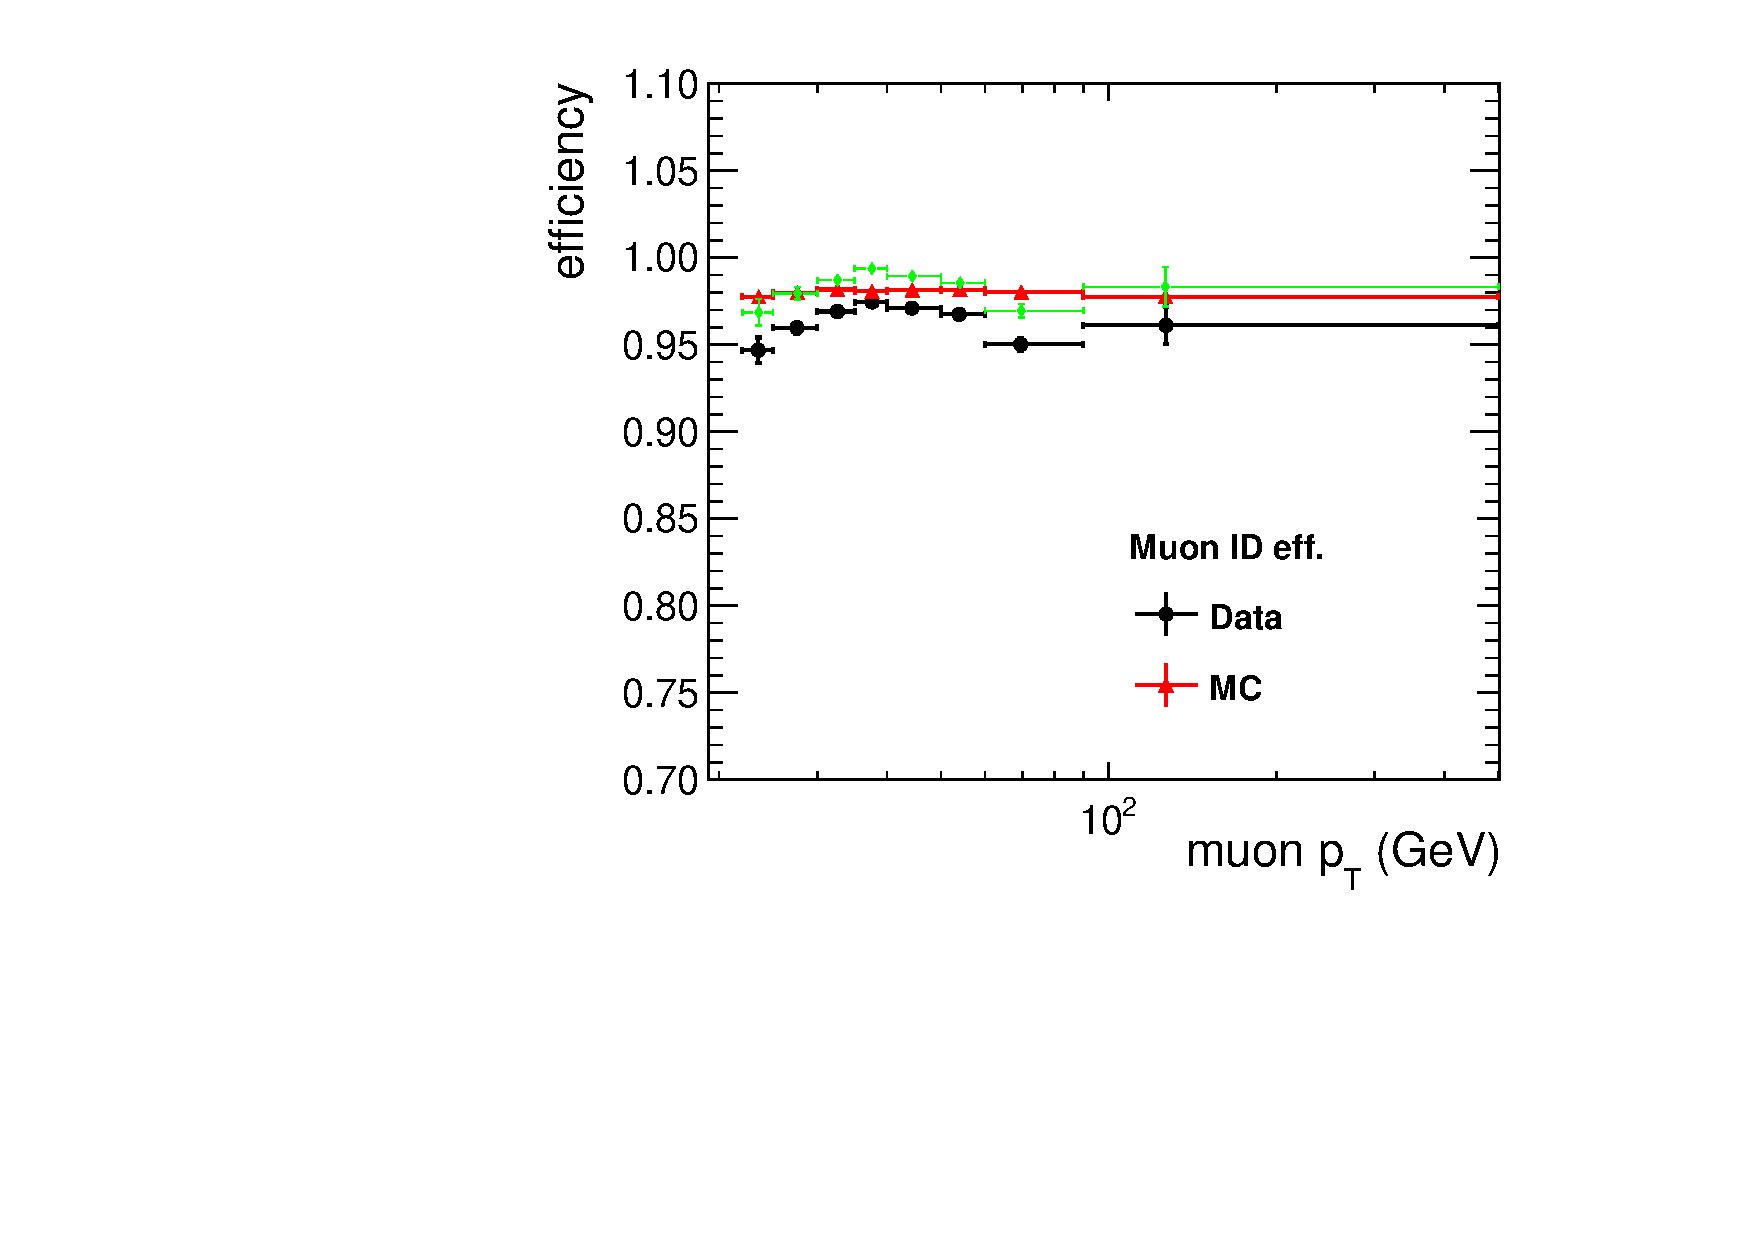
\includegraphics{figures/Figures_MuonEff/muon_ID_pt}}
    \resizebox{0.48 \textwidth}{!}{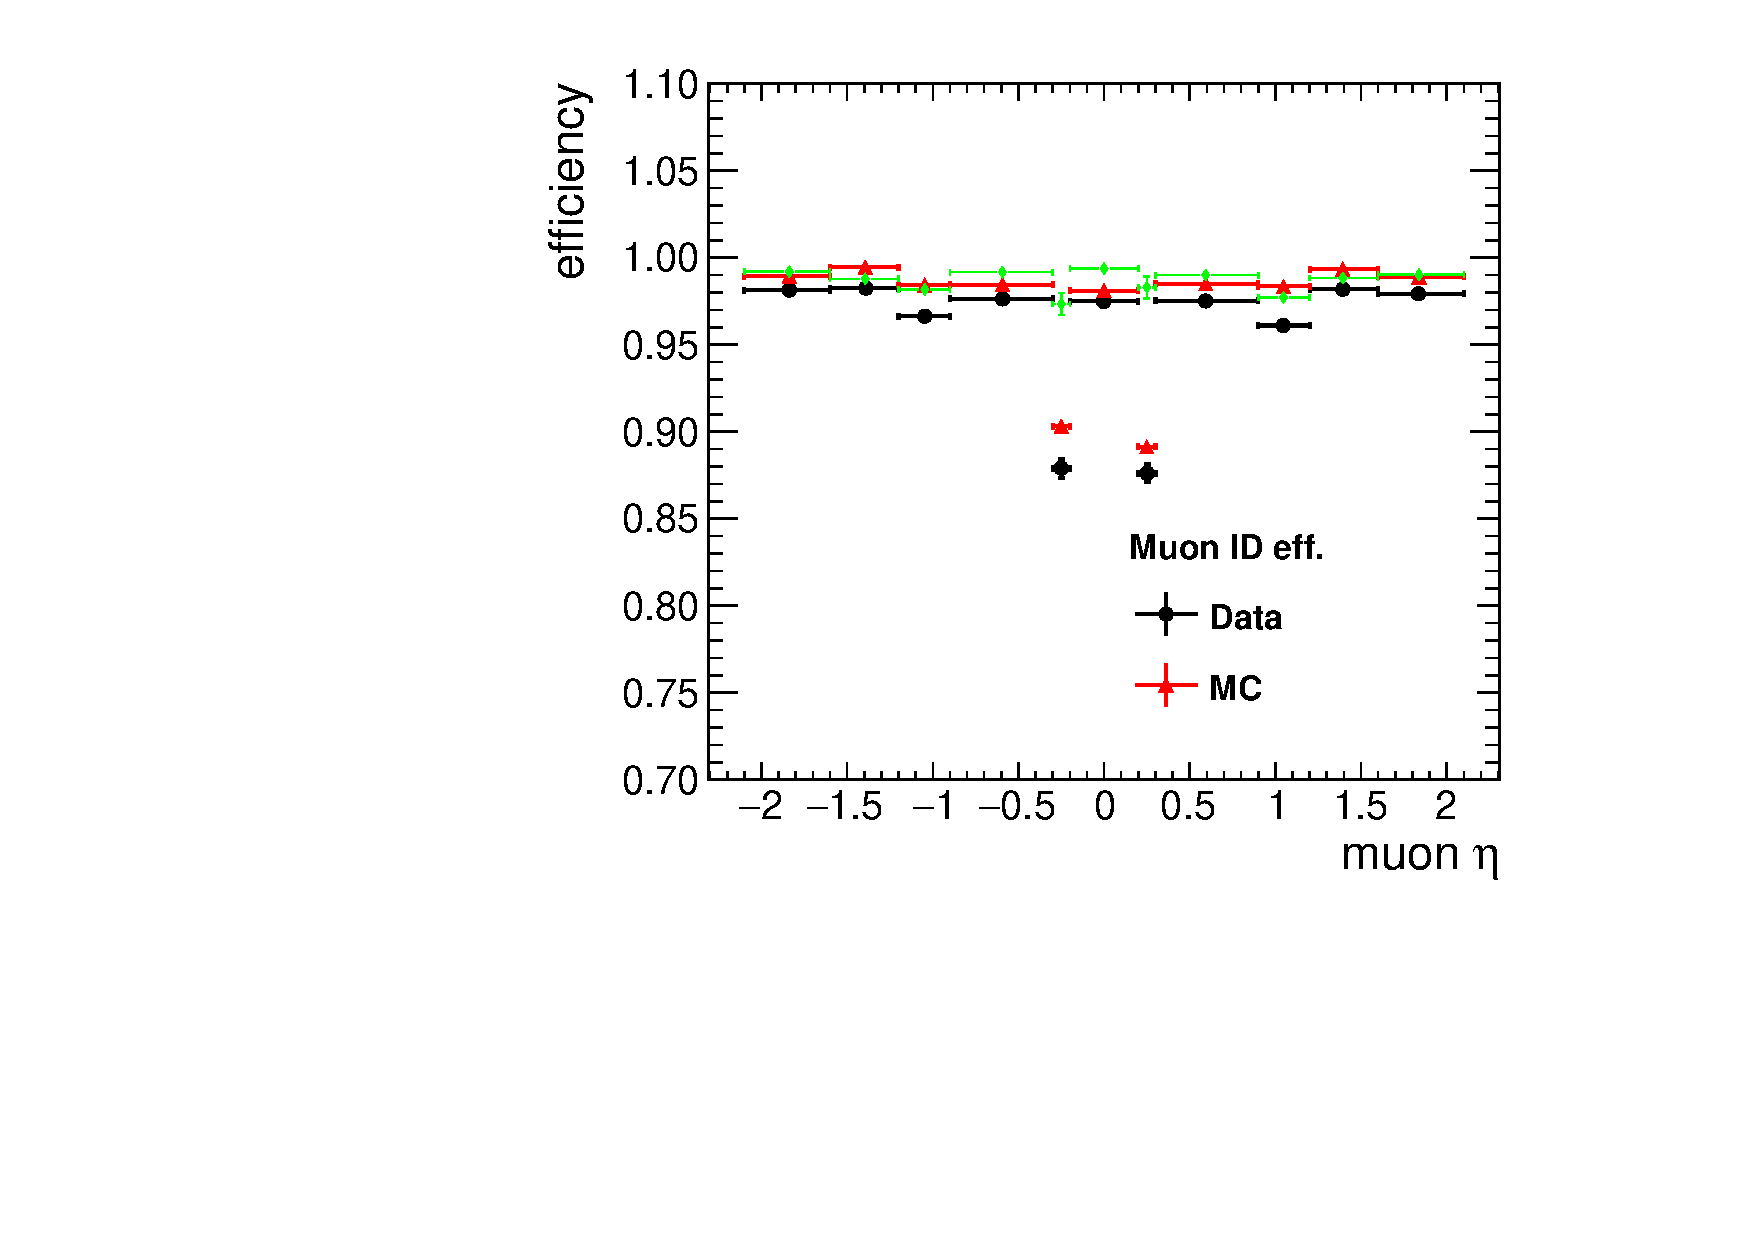
\includegraphics{figures/Figures_MuonEff/muon_ID_eta}}
      \caption{Muon identification efficiency (tight muon definition) in data (black), MC (red) and data-to-MC
        scale factors (green) as a function of muon \pt (left) and $\eta$ (right). Uncertainties are statistical only.}
\label{fig:muonEff_ID}
  \end{center}
\end{figure}


\begin{figure}[htbp!]
  \begin{center}
    \resizebox{0.48 \textwidth}{!}{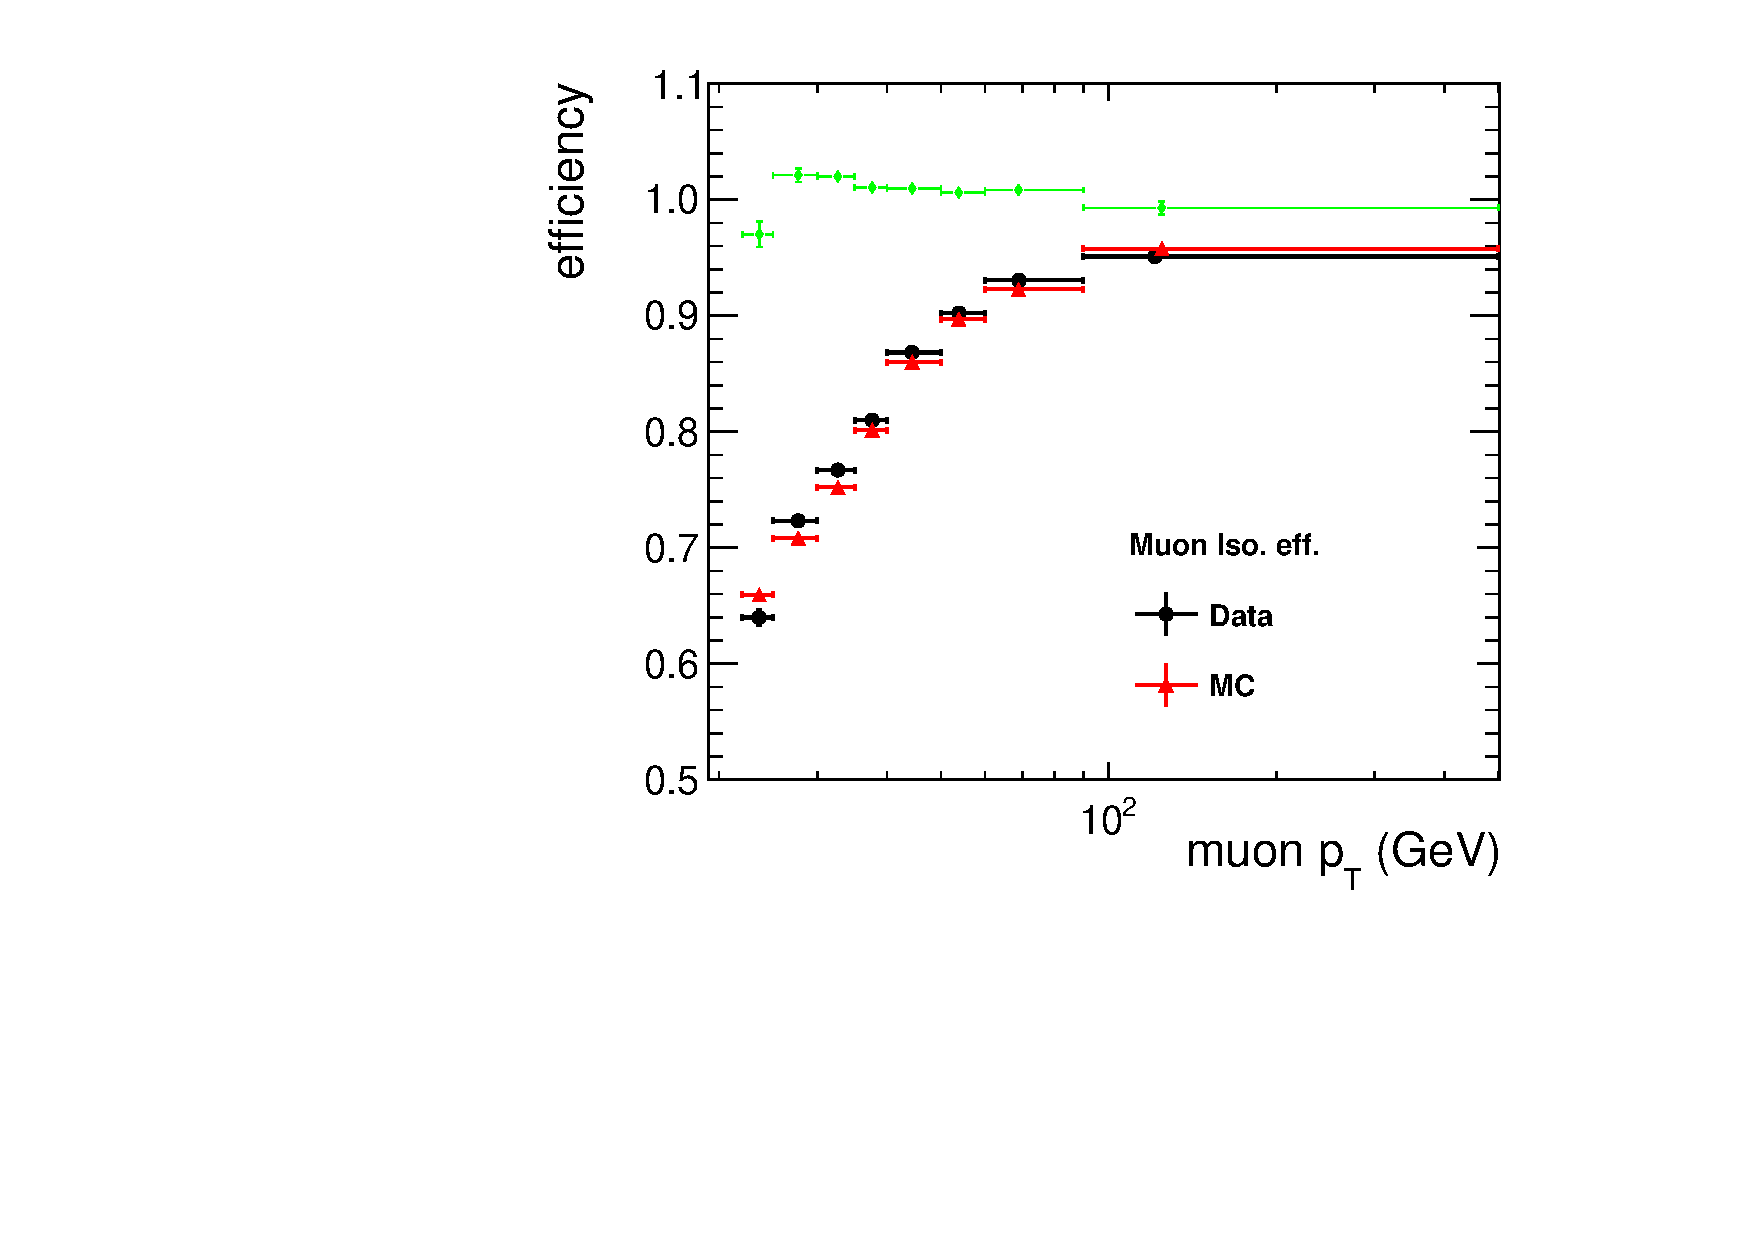
\includegraphics{figures/Figures_MuonEff/muon_Iso_pt}}
    \resizebox{0.48 \textwidth}{!}{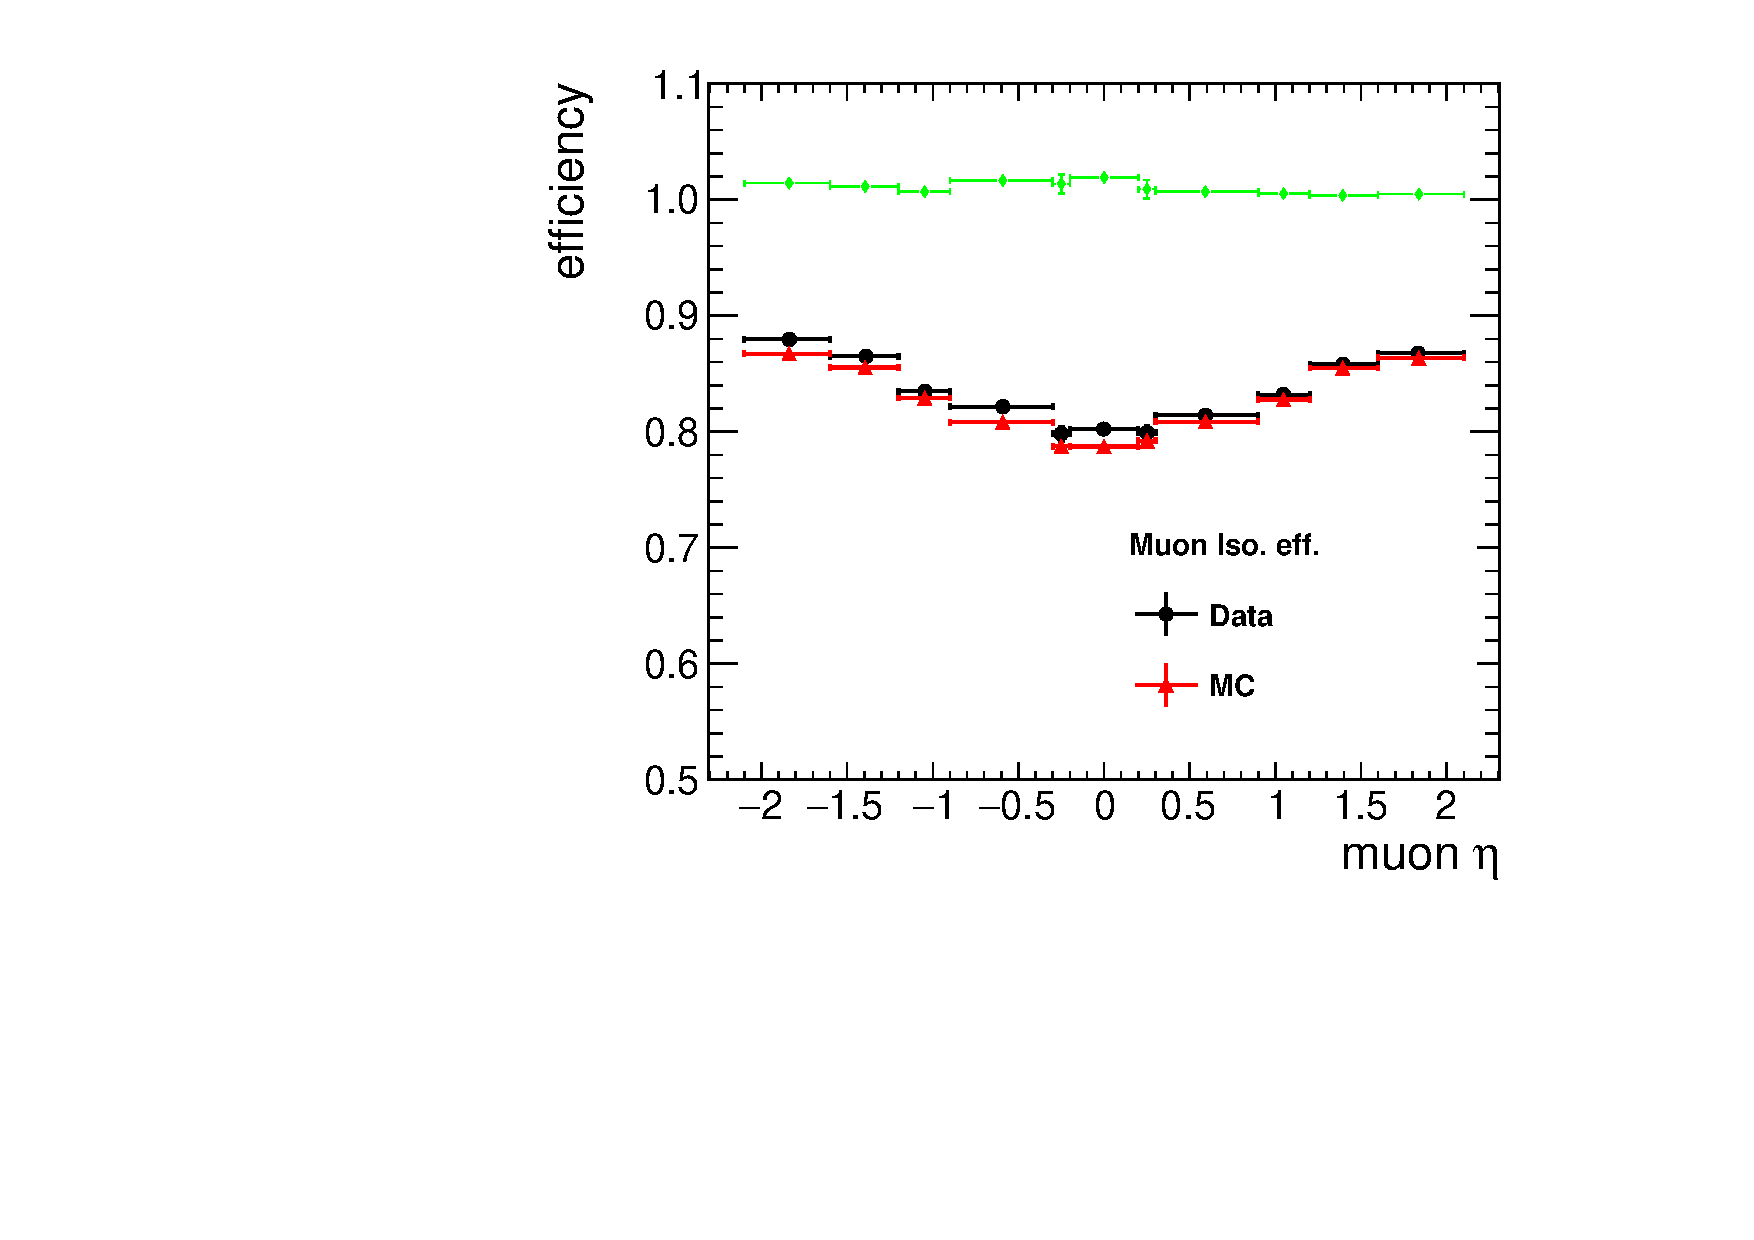
\includegraphics{figures/Figures_MuonEff/muon_Iso_eta}}
      \caption{Muon isolation efficiency in data (black), MC (red) and data-to-MC
        scale factors (green) as a function of muon $\pt$ (left) and $\eta$ (right). Uncertainties are statistical only.}
\label{fig:muonEff_Iso}
  \end{center}
\end{figure}


Systematic uncertainties are estimated by varying the tag muon selection, the signal and background pdfs and the invariant mass window for the fit, and reapplying the tag and probe method. The largest variation of the scale factors with respect to their nominal values is taken as uncertainty of the scale factors. Additional uncertainty is also considered accounting  for the different topology of leptons coming from top decays and Z boson decays. A systematic uncertainty of 1$\%$ is applied on the muon ID scale factors, and between 1.5$\%$ and 2.5$\%$ (depending on the bin) on the isolation scale factors.
%To take into account the different topology of leptons coming from the top decay and Z decays, a more conservative systematic uncertainty of 2\% (preliminary) is used for the global values. 
Figure~\ref{fig:topSFmu1} shows the scale factors as a function of $(|\eta|,p_T)$ of the muon, which are used to correct the MC predictions in the analysis.

\begin{figure}[htbp!]
  \begin{center}
      \resizebox{ \textwidth}{!}{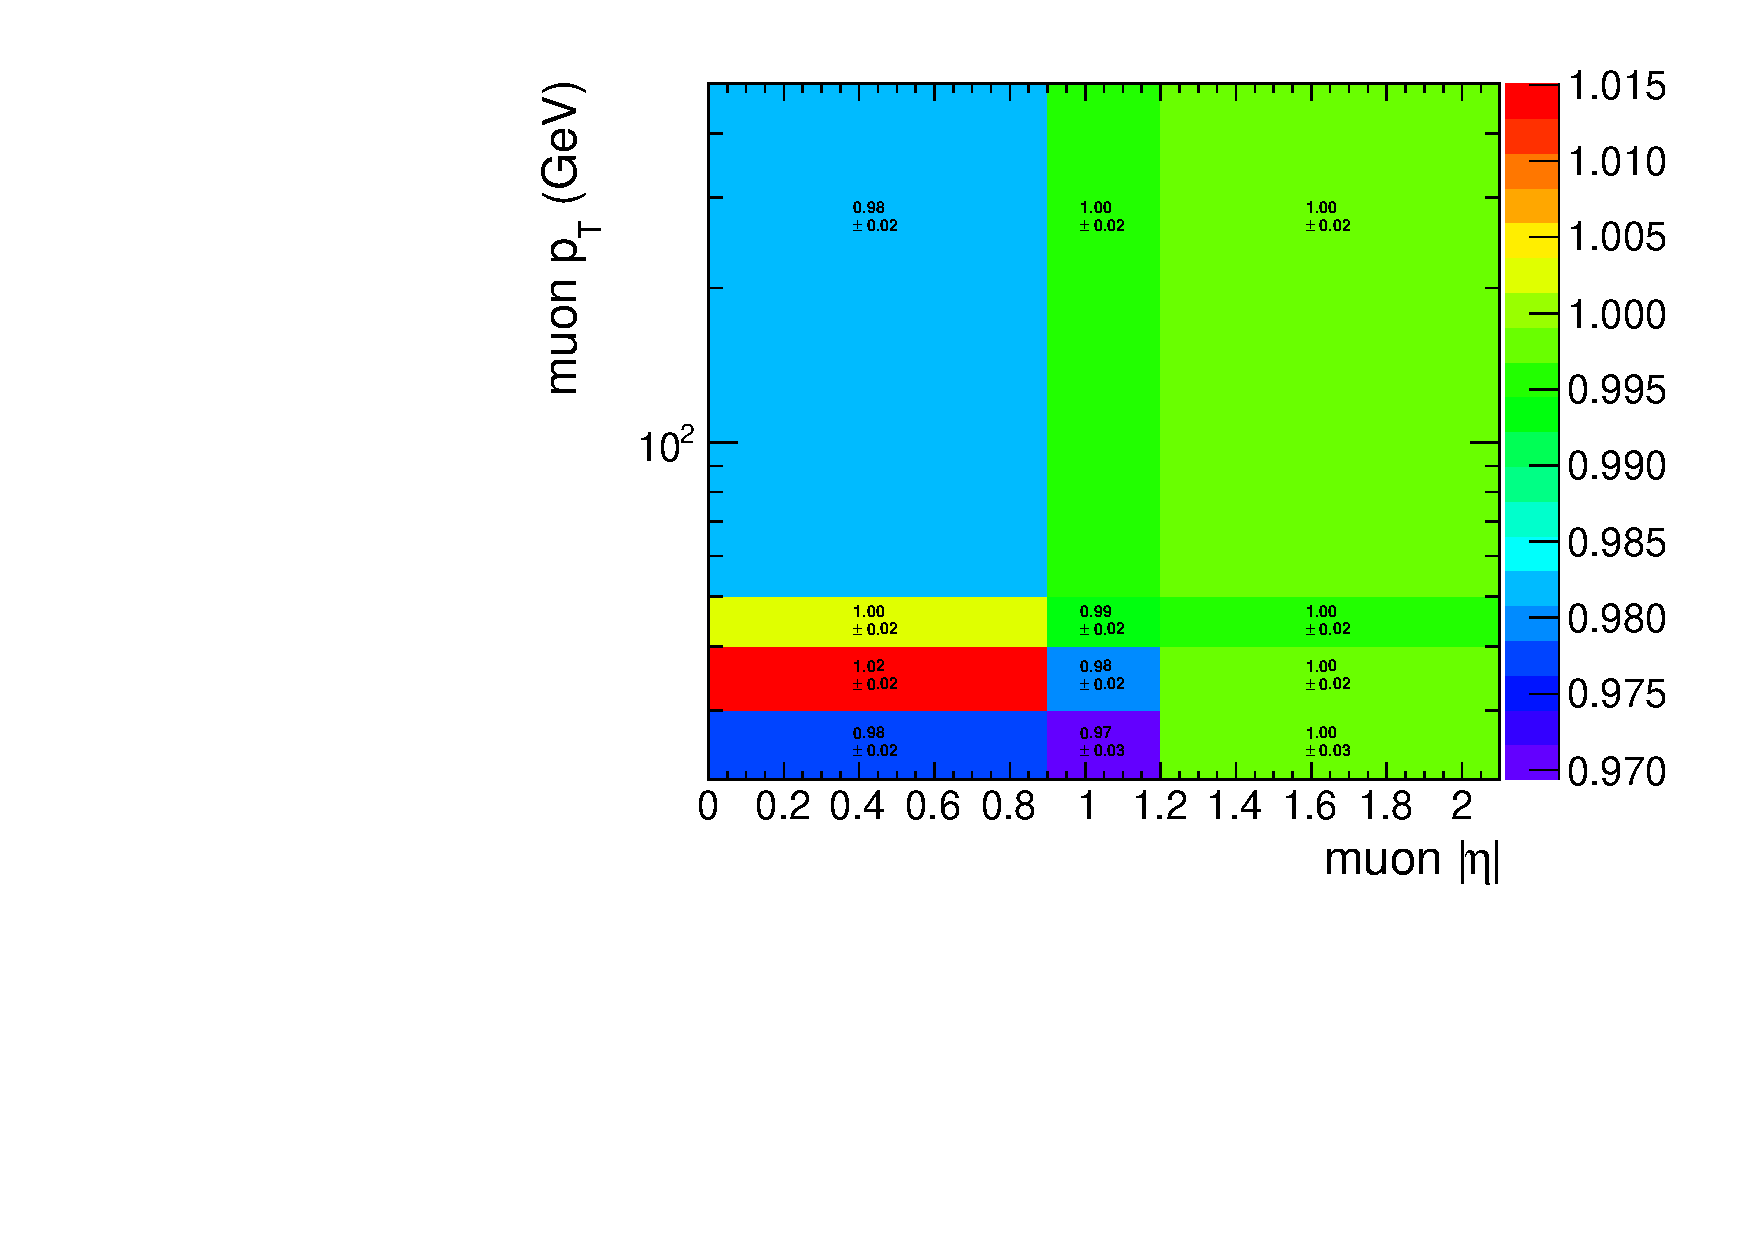
\includegraphics[width=1.1\textwidth]{figures/Figures_MuonEff/muon_IDxIso_2d.pdf}}%
  \end{center}
   \caption{Scale factors accounting for Identification x Isolation efficiencies as a function of ($|\eta|$, p$_T$) of muons. The uncertainties in the plot correspond to the  statistical and systematic uncertainties added in quadrature. The scale factors are in the range 0.97-1.02 and the total uncertainties are of the order of 2-3$\%$ in the different bins.}
  \label{fig:topSFmu1}
\end{figure}






%%%%%%%%%%%%%%%%%%%%%%%%%%%%%%%%%
\subsection{High level trigger efficiency}
\label{subsec:hlt}
To maximize the trigger efficiency, the trigger bit ''HLT\_IsoMu20\_eta2p1'' is combined through a logical ''OR'' with the bit ''HLT\_IsoTkMu20\_eta2p1'' which uses a tracker muon HLT algorithm. 
The efficiency of ''HLT\_IsoMu20\_eta2p1 OR HLT\_IsoTkMu20\_eta2p1'' is also measured with the tag and probe method as described in Section \ref{sec:muonEff1}. The same tag muon selection is used as in the ID and isolation efficiency measurement. The probe muons pass the full lepton selection  used in the analysis, the passing probe muons in addition are matched to the trigger bit of interest. The measured single muon efficiencies and scale factors are shown in Figure~\ref{fig:muonEff_HLT_IsoMu20}. Figure~\ref{fig:topSFmu2} shows the scale factors as a function of $(|\eta|,p_T)$ of the muon, which are used to correct the MC predictions in the analysis. The estimated systematic uncertainty of the scale factors is of the order of 1-1.5$\%$.

\begin{figure}[htbp!]
  \begin{center}
    \resizebox{0.48 \textwidth}{!}{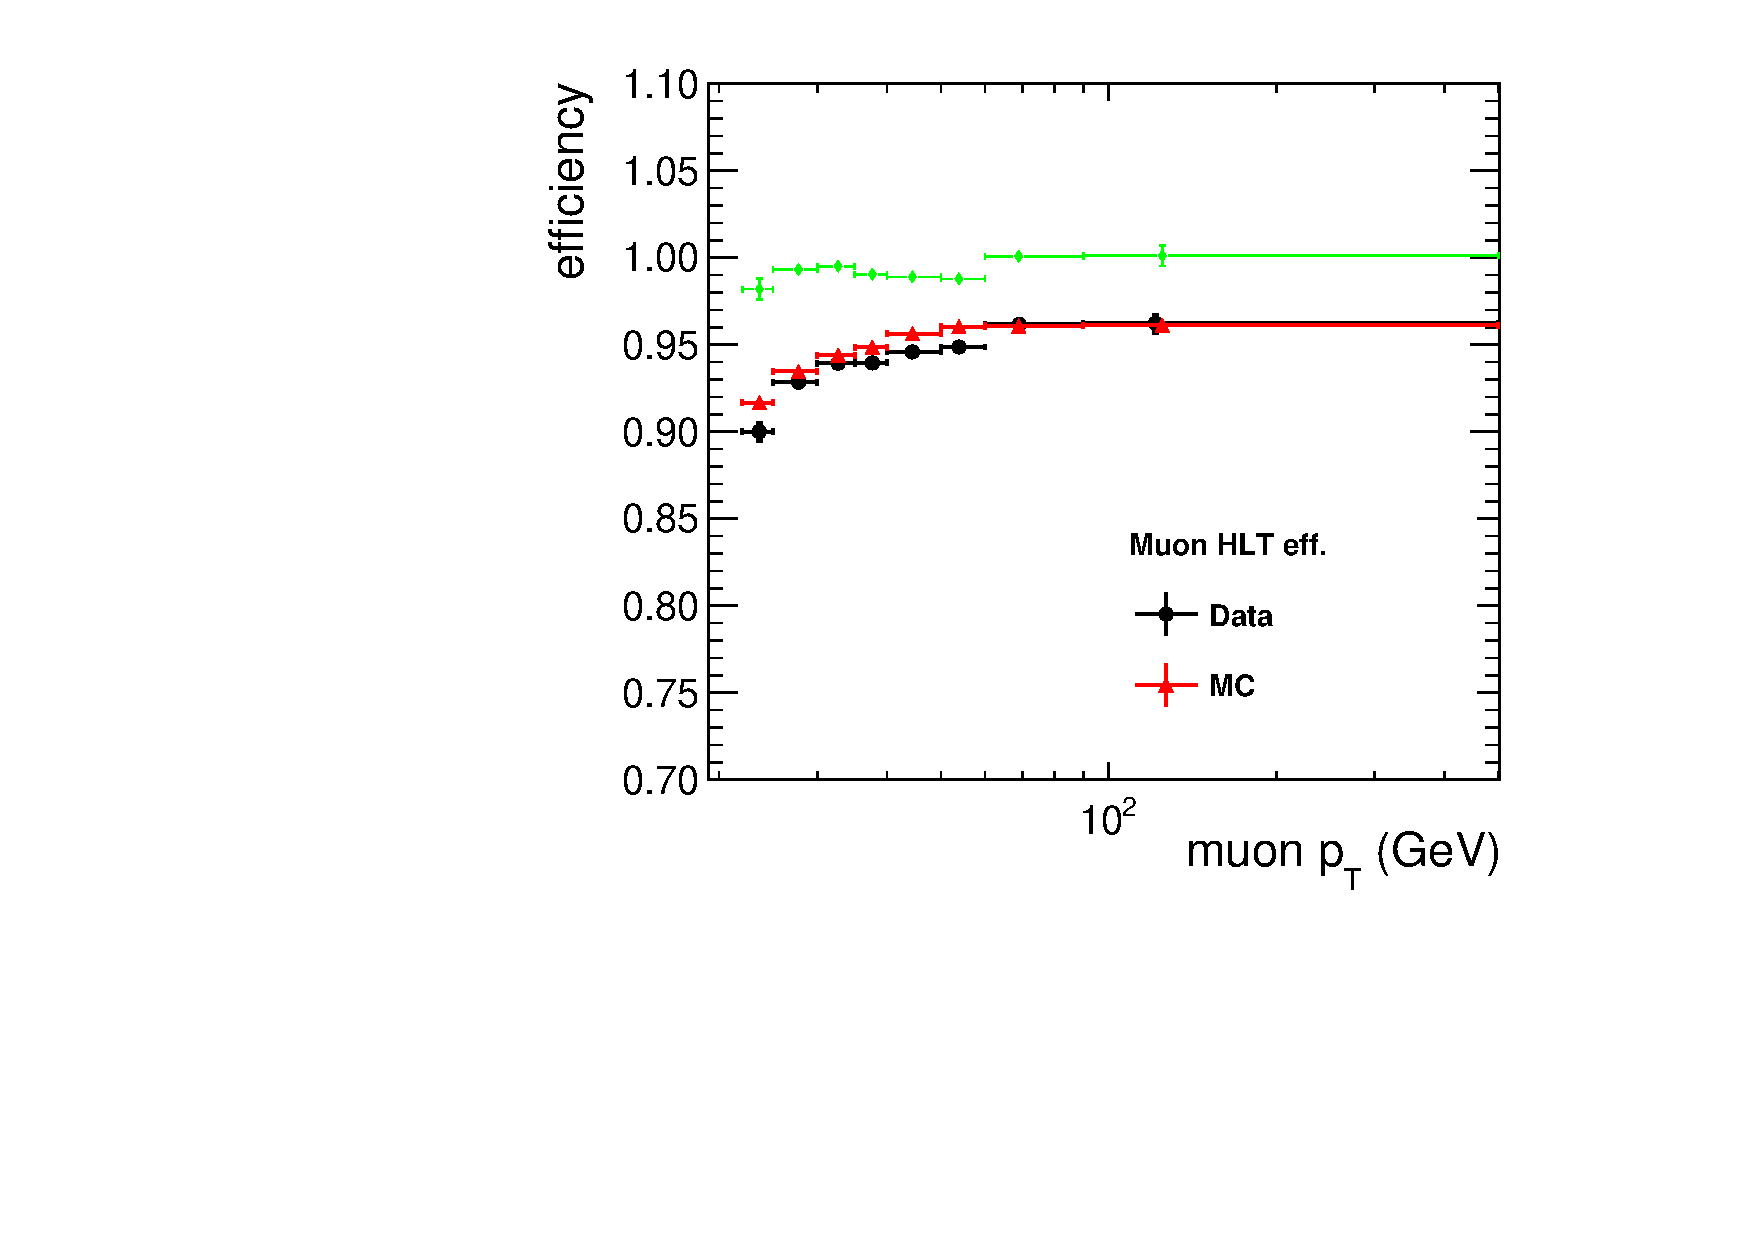
\includegraphics{figures/Figures_MuonEff/muon_HLT_pt}}
    \resizebox{0.48 \textwidth}{!}{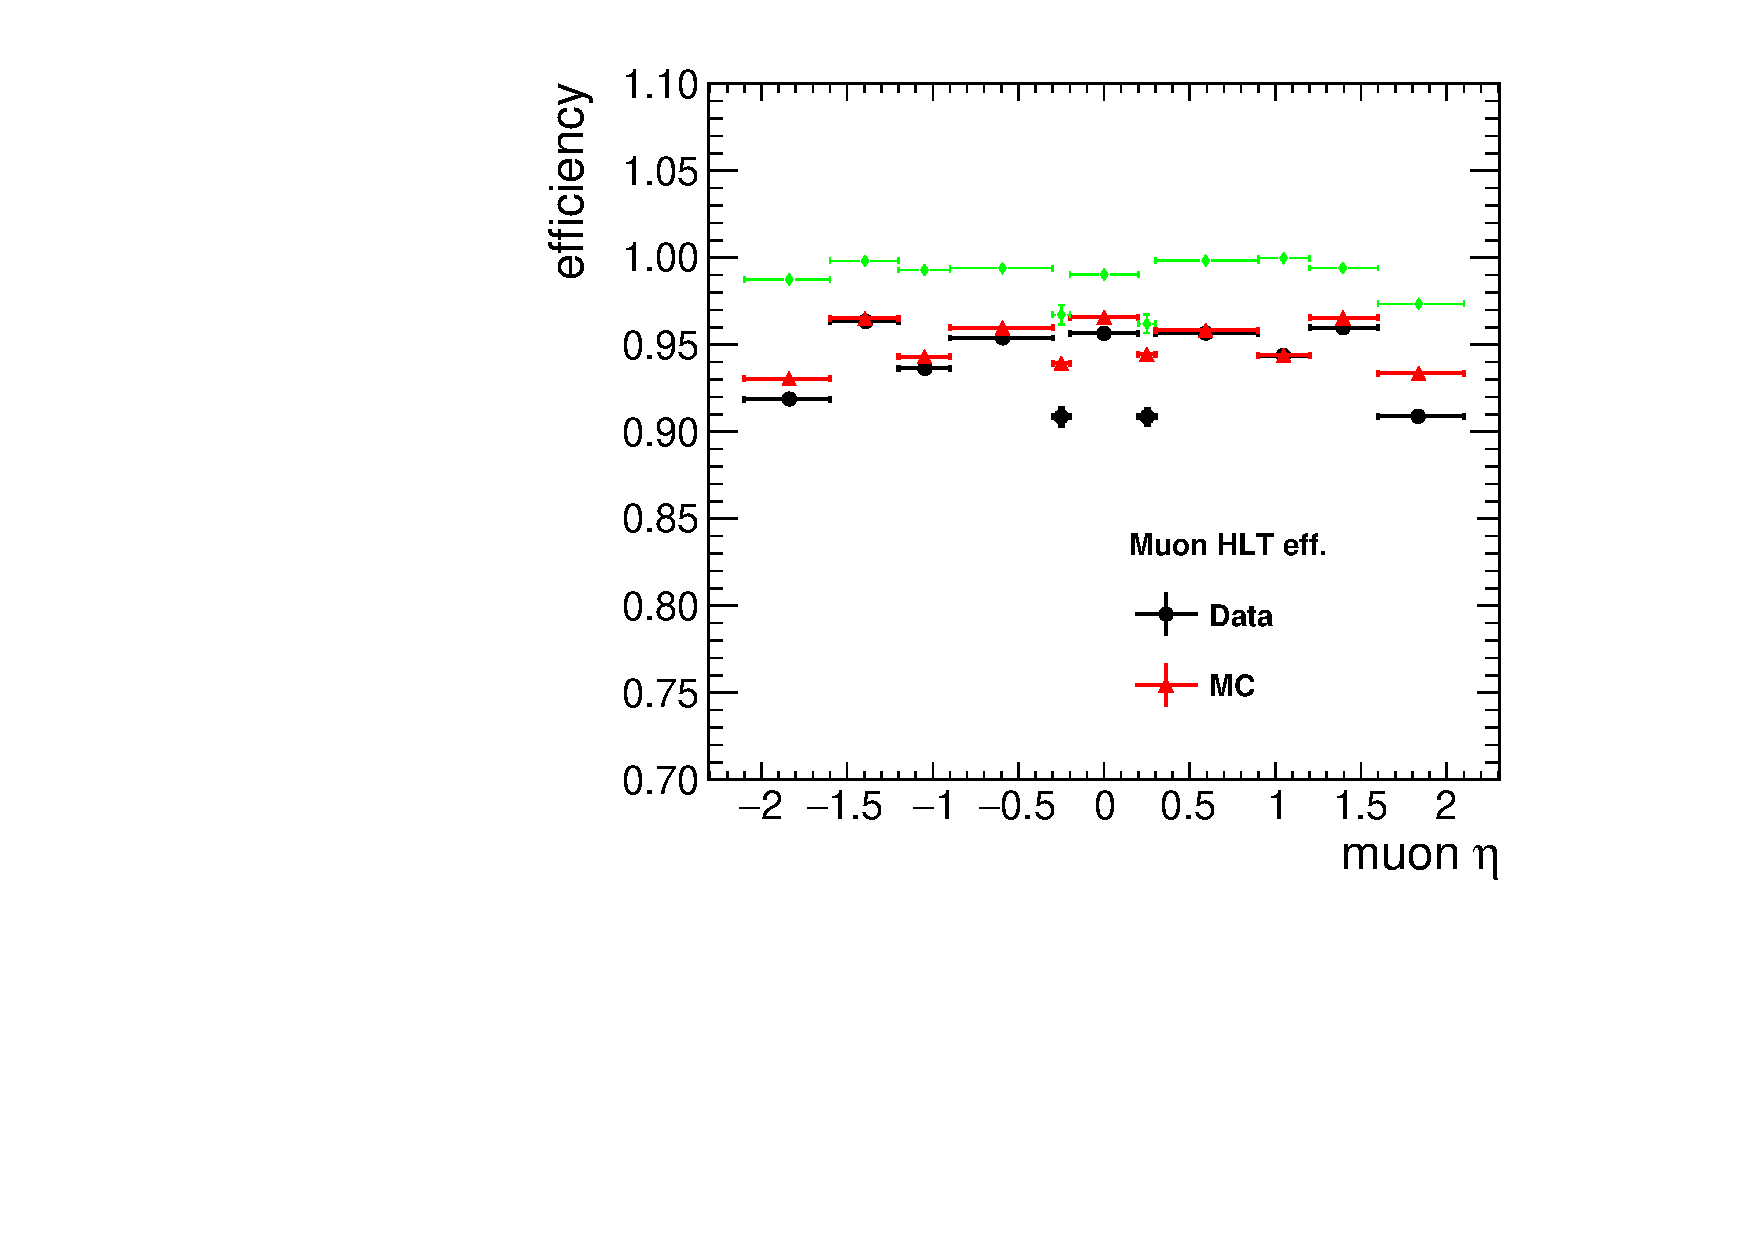
\includegraphics{figures/Figures_MuonEff/muon_HLT_eta}}
      \caption{Efficiency of the single muon triggers ''HLT\_IsoMu20\_eta2p1 OR HLT\_IsoTkMu20\_eta2p1'' for data (black), MC (red) and data-to-MC
        scale factors (green) as a function of muon $\pt$ (left) and $\eta$ (right). Uncertainties are statistical only.}
\label{fig:muonEff_HLT_IsoMu20}
  \end{center}
\end{figure}



\begin{figure}[htbp!]
  \begin{center}
   \resizebox{ \textwidth}{!}{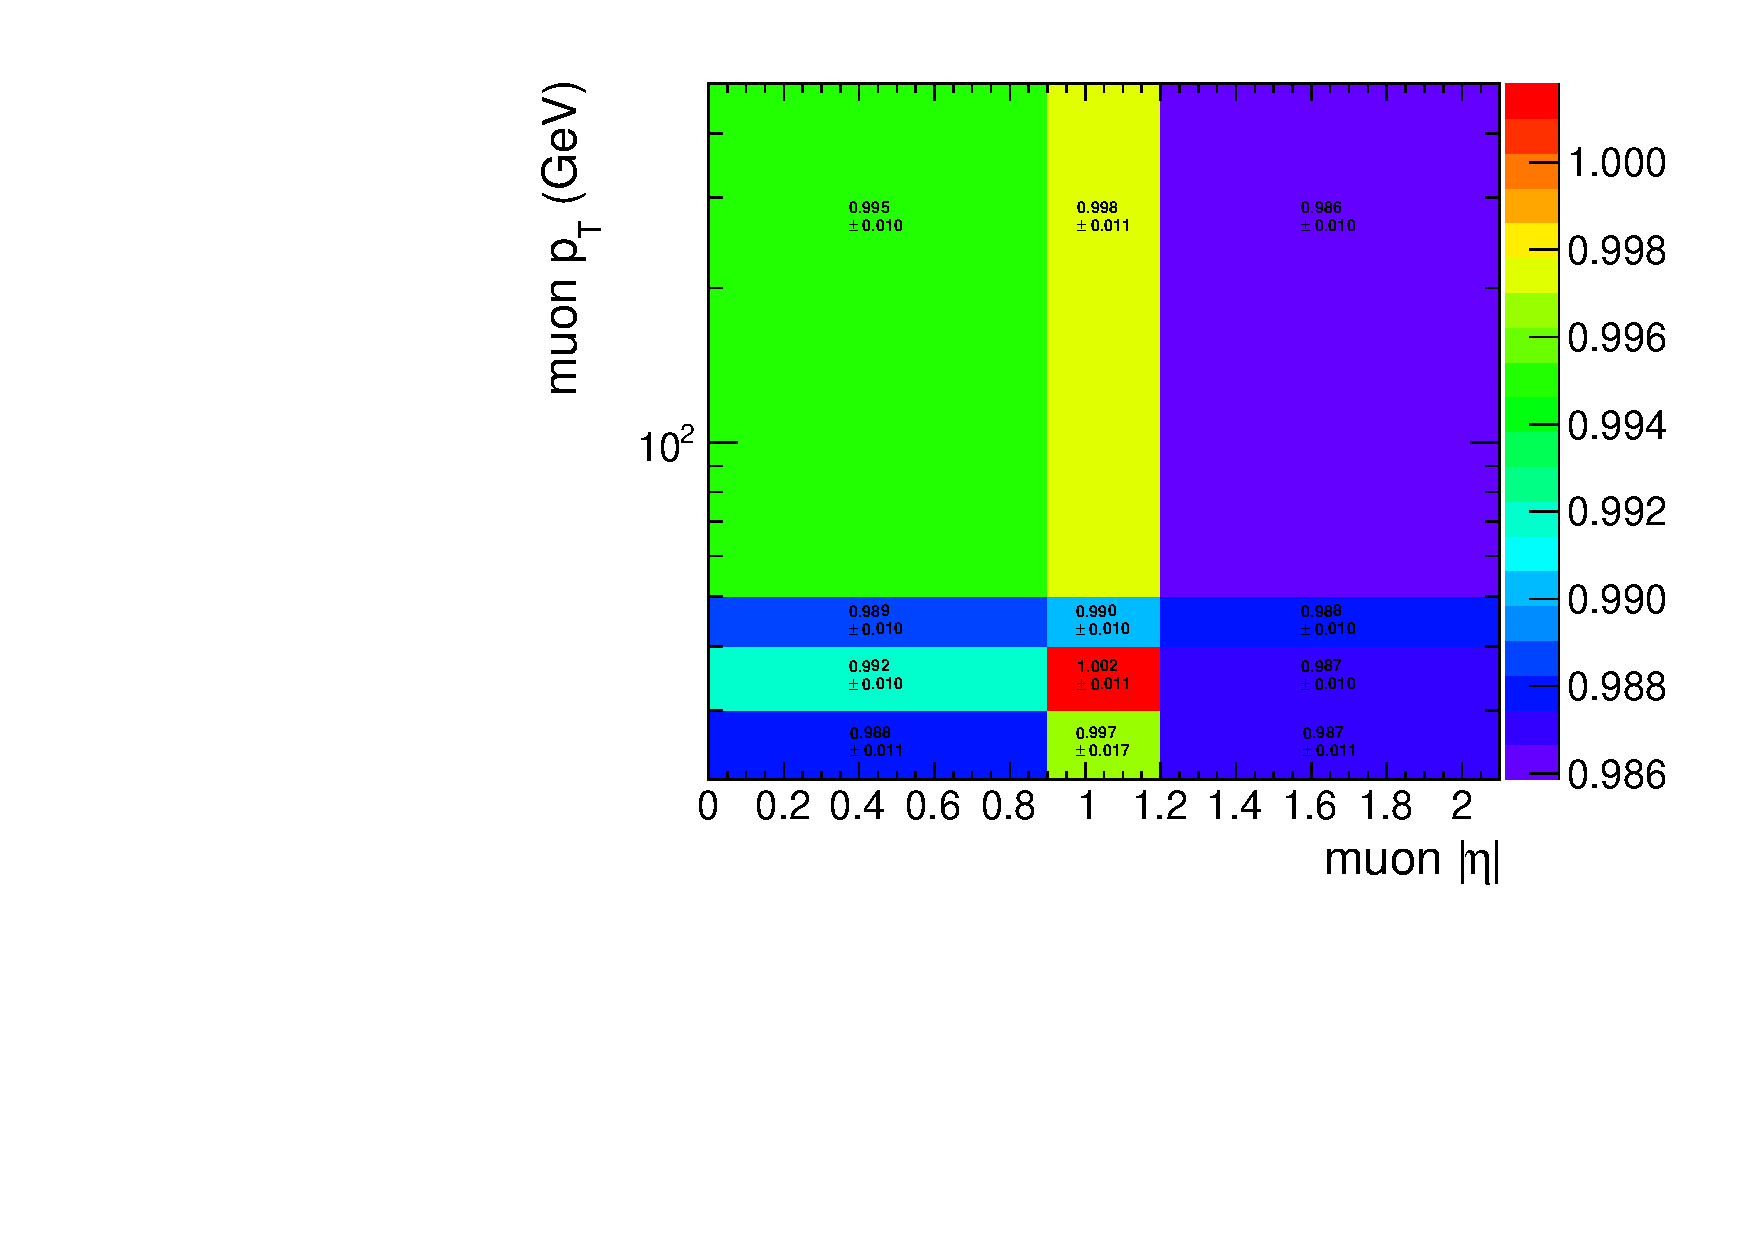
\includegraphics[width=1.2\textwidth]{figures/Figures_MuonEff/muon_HLT_2d}}%
  \end{center}
   \caption{Data-to-MC scale factors accounting for ''HLT\_IsoMu20\_eta2p1 OR HLT\_IsoTkMu20\_eta2p1'' efficiency. The uncertainties in the plot correspond to the  statistical and systematic uncertainties added in quadrature. The scale factors are in the range 0.98-1.00 and the uncertainties are of the order of 1-2$\%$.}
  \label{fig:topSFmu2}
\end{figure}


